\documentclass[11pt,a4paper]{article}

% ============================================================
% Packages
% ============================================================

\usepackage[utf8]{inputenc}
\usepackage[T1]{fontenc}
\usepackage{lmodern}
\usepackage{geometry}
\usepackage{amsmath, amssymb, amsthm, mathtools}
\usepackage{booktabs}
\usepackage{array}
\usepackage{longtable}
\usepackage{enumitem}
\usepackage{hyperref}
\usepackage{xcolor}
\usepackage{tikz}
\usepackage{caption}
\usepackage{float}

\usetikzlibrary{
    arrows.meta,
    positioning,
    shapes.geometric,
    fit,
    calc
}

\geometry{margin=25mm}

\hypersetup{
    colorlinks=true,
    linkcolor=blue,
    citecolor=blue,
    urlcolor=blue
}

% ============================================================
% Theorem-like environments
% ============================================================

\newtheorem{definition}{Definition}
\newtheorem{principle}{Principle}
\newtheorem{proposition}{Proposition}
\newtheorem{remark}{Remark}

% ============================================================
% Custom commands
% ============================================================

\newcommand{\MG}{\mathrm{MG}}
\newcommand{\GO}{\mathrm{GO}}
\newcommand{\HOLD}{\mathrm{HOLD}}
\newcommand{\REPAIR}{\mathrm{REPAIR}}
\newcommand{\BLOCK}{\mathrm{BLOCK}}
\newcommand{\PASS}{\mathrm{PASS}}
\newcommand{\VIOLATION}{\mathrm{VIOLATION}}
\newcommand{\OBSERVE}{\mathrm{OBSERVE}}
\newcommand{\PAUSE}{\mathrm{PAUSE}}
\newcommand{\ROLLBACK}{\mathrm{ROLLBACK}}
\newcommand{\ESCALATE}{\mathrm{ESCALATE}}
\newcommand{\FGR}{\mathrm{FGR}}
\newcommand{\PVR}{\mathrm{PVR}}

% ============================================================
% TikZ styles
% ============================================================

\tikzset{
    block/.style={
        rectangle,
        rounded corners,
        draw=black,
        very thick,
        align=center,
        minimum height=9mm,
        minimum width=35mm,
        font=\small
    },
    smallblock/.style={
        rectangle,
        rounded corners,
        draw=black,
        thick,
        align=center,
        minimum height=8mm,
        minimum width=28mm,
        font=\scriptsize
    },
    decision/.style={
        diamond,
        draw=black,
        thick,
        align=center,
        aspect=2.2,
        inner sep=1.5pt,
        font=\scriptsize
    },
    arrow/.style={
        -{Latex[length=3mm]},
        thick
    },
    dashedbox/.style={
        rectangle,
        rounded corners,
        draw=black,
        dashed,
        thick,
        inner sep=5pt
    }
}

% ============================================================
% Title
% ============================================================

\title{
\textbf{I2OS Mini Gate:}\\
A Formal Model of Runtime Transition Governance\\
with Diagrams and Tables\\
\large From v0.1 to the v4.1 Design Stage
}

\author{
Masayuki Ando / ANDOM\\
Independent Researcher, Japan
}

\date{\today}

\begin{document}

\maketitle

% ============================================================
% Abstract
% ============================================================

\begin{abstract}
Modern AI safety frameworks often focus on output filtering, alignment, reward optimization, or post-hoc evaluation.
However, as AI systems increasingly interact with tools, files, APIs, memory, and external environments, safety must be extended from output-level control to action-level governance.

This paper presents a formal model of \textit{I2OS Mini Gate}, a compact runtime governance system developed from version v0.1 to the v4.1 design stage.
I2OS Mini Gate treats proposed AI or software actions as state transitions before execution.
It classifies them as \(\GO\), \(\HOLD\), \(\REPAIR\), or \(\BLOCK\), converts permitted transitions into bounded execution contracts, enforces those contracts during attempted execution, and responds to contract violations through severity classification, containment, repair, rollback, escalation, blocking, and human-verifiable reporting.

The core principle is:

\[
\mathrm{Capability} \neq \mathrm{Permission}.
\]

The resulting model frames AI safety as pre-execution transition governance, bounded permission during execution, and structured response after violation.
\end{abstract}

\textbf{Keywords:} AI Safety, Runtime Governance, Transition Governance, Admissibility, Execution Contract, Agentic AI, I2OS, Human-Verifiable Governance

\newpage
\tableofcontents
\newpage

% ============================================================
\section{Introduction}

AI systems are moving from passive text generation toward action-oriented execution.
Modern systems may read and write files, call external APIs, send messages, execute commands, modify memory, and delegate tasks to other agents.

This shift creates a new safety problem.
It is no longer sufficient to ask whether an AI output is acceptable after generation.
Instead, systems must ask whether a proposed action should become real before execution.

\begin{principle}[Core Principle]
\[
\mathrm{Capability} \neq \mathrm{Permission}.
\]
A system should not execute an action simply because it can.
\end{principle}

The central claim of this paper is that AI safety should be understood not only as output filtering, but as runtime transition governance.

% ============================================================
\section{Evolution of I2OS Mini Gate}

I2OS Mini Gate evolved from a minimal classifier into a closed-loop runtime governance prototype.

\begin{figure}[H]
\centering
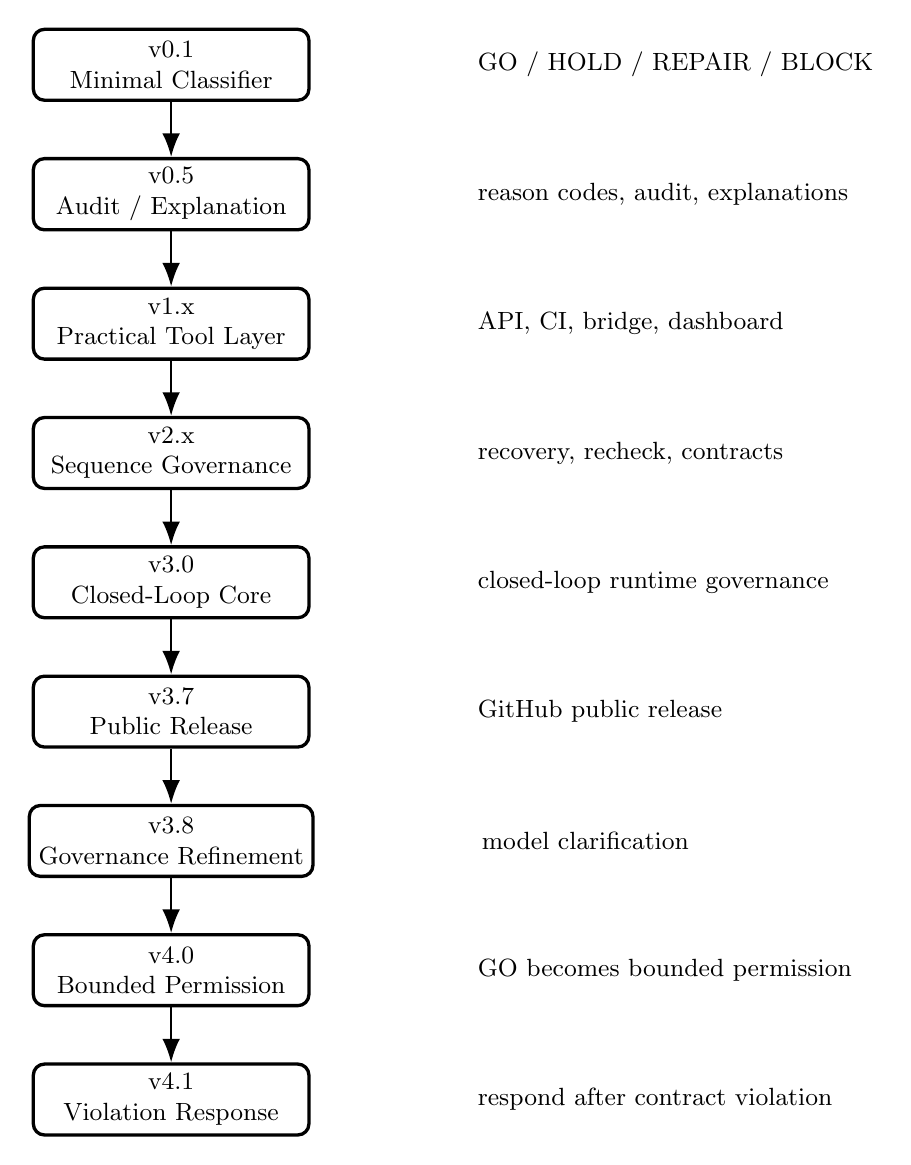
\begin{tikzpicture}[node distance=7mm]

\node[block] (v01) {v0.1\\Minimal Classifier};
\node[block, below=of v01] (v05) {v0.5\\Audit / Explanation};
\node[block, below=of v05] (v1) {v1.x\\Practical Tool Layer};
\node[block, below=of v1] (v2) {v2.x\\Sequence Governance};
\node[block, below=of v2] (v3) {v3.0\\Closed-Loop Core};
\node[block, below=of v3] (v37) {v3.7\\Public Release};
\node[block, below=of v37] (v38) {v3.8\\Governance Refinement};
\node[block, below=of v38] (v40) {v4.0\\Bounded Permission};
\node[block, below=of v40] (v41) {v4.1\\Violation Response};

\draw[arrow] (v01) -- (v05);
\draw[arrow] (v05) -- (v1);
\draw[arrow] (v1) -- (v2);
\draw[arrow] (v2) -- (v3);
\draw[arrow] (v3) -- (v37);
\draw[arrow] (v37) -- (v38);
\draw[arrow] (v38) -- (v40);
\draw[arrow] (v40) -- (v41);

\node[right=20mm of v01, align=left, font=\small] {GO / HOLD / REPAIR / BLOCK};
\node[right=20mm of v05, align=left, font=\small] {reason codes, audit, explanations};
\node[right=20mm of v1, align=left, font=\small] {API, CI, bridge, dashboard};
\node[right=20mm of v2, align=left, font=\small] {recovery, recheck, contracts};
\node[right=20mm of v3, align=left, font=\small] {closed-loop runtime governance};
\node[right=20mm of v37, align=left, font=\small] {GitHub public release};
\node[right=20mm of v38, align=left, font=\small] {model clarification};
\node[right=20mm of v40, align=left, font=\small] {GO becomes bounded permission};
\node[right=20mm of v41, align=left, font=\small] {respond after contract violation};

\end{tikzpicture}
\caption{Evolutionary roadmap of I2OS Mini Gate from v0.1 to v4.1.}
\end{figure}

\begin{longtable}{p{0.16\linewidth} p{0.28\linewidth} p{0.46\linewidth}}
\toprule
\textbf{Version} & \textbf{Role} & \textbf{Structural Meaning} \\
\midrule
v0.1 & Minimal Gate Prototype & Introduced \(\GO / \HOLD / \REPAIR / \BLOCK\) classification. \\
v0.5 & Audit and Explanation & Added reason codes, risk levels, logs, and human-verifiable explanations. \\
v1.x & Practical Tool Layer & Added API mode, CI hooks, agent runtime bridge, prompt-injection tests, dashboard, and error handling. \\
v2.x & Sequence Governance & Extended from single-action checks to recovery paths, recheck loops, execution contracts, and enforcement. \\
v3.0 & Closed-Loop Governance Core & Integrated human-admissibility, recovery, recheck, contract generation, enforcement, and final reporting. \\
v3.7 & Public Release Stabilization & Prepared the repository for public GitHub release. \\
v3.8 & Runtime Governance Refinement & Clarified the transition governance model and example cases. \\
v4.0 & Stable Closed-Loop Runtime Governance & Introduced bounded permission through execution contracts. \\
v4.1 & Contract Violation Response & Defined structured responses when execution violates a contract. \\
\bottomrule
\end{longtable}

The structural trajectory is:

\[
\text{Classifier}
\rightarrow
\text{Explainer}
\rightarrow
\text{Tool}
\rightarrow
\text{Sequence Governor}
\rightarrow
\text{Closed-Loop Runtime Governance}
\rightarrow
\text{Bounded Permission}
\rightarrow
\text{Violation Response}.
\]

% ============================================================
\section{State Transition Model}

Let \(S_t\) denote the current state of the system.
Let \(T\) denote a proposed AI or software action.
Let \(S_{t+1}\) denote the predicted next state after the transition.

A proposed action is modeled as a state transition:

\[
T : S_t \rightarrow S_{t+1}.
\]

The fundamental question is:

\[
\text{Should } T \text{ be permitted before execution?}
\]

\begin{figure}[H]
\centering
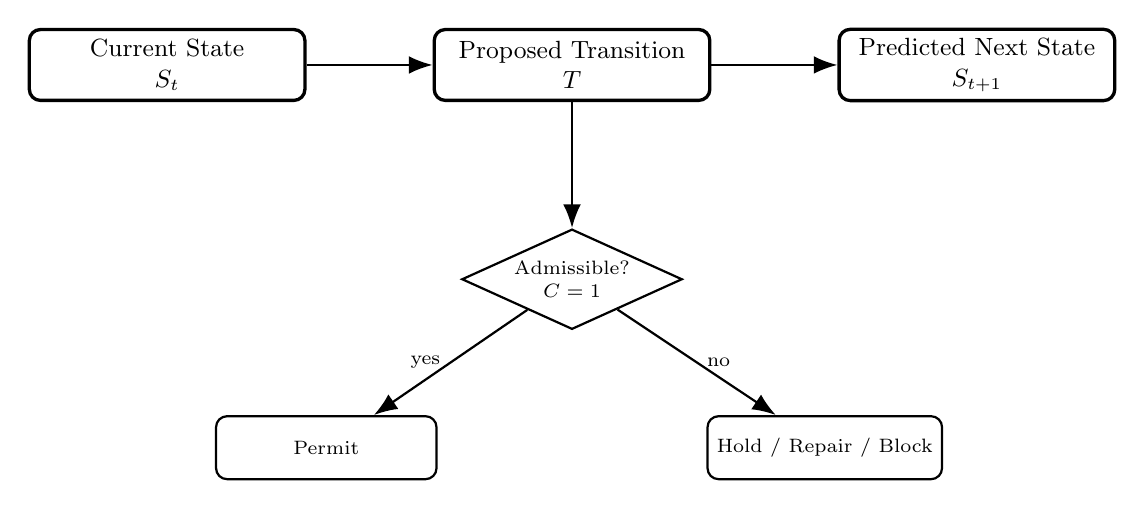
\begin{tikzpicture}[node distance=16mm]
\node[block] (s0) {Current State\\\(S_t\)};
\node[block, right=of s0] (t) {Proposed Transition\\\(T\)};
\node[block, right=of t] (s1) {Predicted Next State\\\(S_{t+1}\)};
\node[decision, below=of t] (c) {Admissible?\\\(C=1\)};
\node[smallblock, below left=14mm and 10mm of c] (permit) {Permit};
\node[smallblock, below right=14mm and 10mm of c] (reject) {Hold / Repair / Block};

\draw[arrow] (s0) -- (t);
\draw[arrow] (t) -- (s1);
\draw[arrow] (t) -- (c);
\draw[arrow] (c) -- node[left, font=\scriptsize] {yes} (permit);
\draw[arrow] (c) -- node[right, font=\scriptsize] {no} (reject);

\end{tikzpicture}
\caption{A proposed action is modeled as a state transition before execution.}
\end{figure}

% ============================================================
\section{Admissibility and the Permit Equation}

\begin{definition}[Admissibility Constraint]
An admissibility constraint \(C\) determines whether a proposed transition preserves recoverable, synchronized, context-valid, future-compatible continuity.
\end{definition}

The core permit equation is:

\[
Permit(T)
=
\mathbf{1}
\left[
C(S_t,T,S_{t+1}) = 1
\right].
\]

Thus:

\[
Permit(T)=1
\]

if and only if the transition from \(S_t\) to \(S_{t+1}\) through \(T\) satisfies the admissibility constraint.

% ============================================================
\section{Admissibility Constraint Decomposition}

The admissibility constraint is multi-layered:

\[
C(S_t,T,S_{t+1})
=
C_{\mathrm{context}}
\land
C_{\mathrm{safety}}
\land
C_{\mathrm{recovery}}
\land
C_{\mathrm{sync}}
\land
C_{\mathrm{future}}
\land
C_{\mathrm{human}}
\land
C_{\mathrm{scope}}
\land
C_{\mathrm{audit}}.
\]

\begin{figure}[H]
\centering
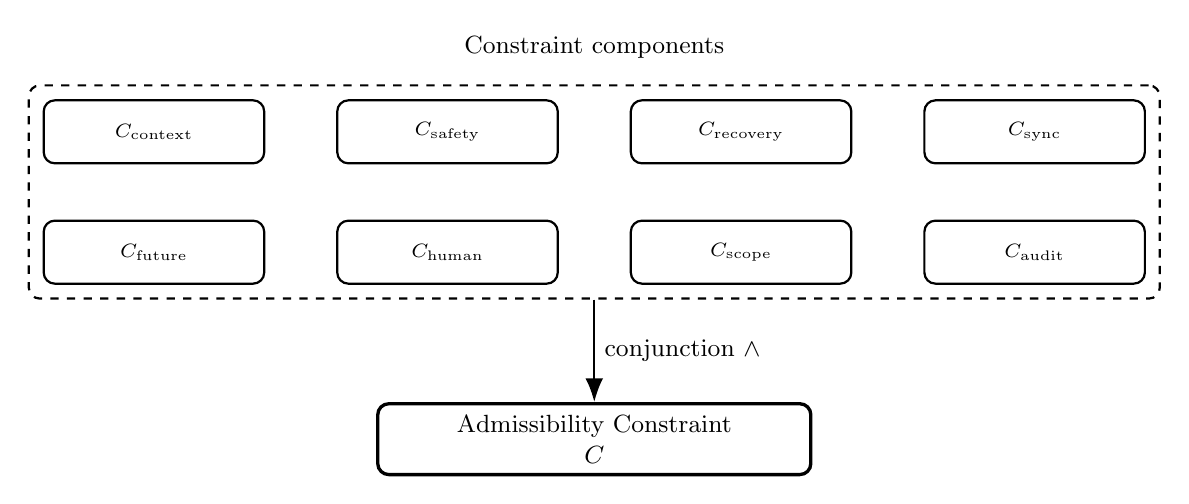
\begin{tikzpicture}[node distance=7mm and 9mm]
\node[smallblock] (context) {\(C_{\mathrm{context}}\)};
\node[smallblock, right=of context] (safety) {\(C_{\mathrm{safety}}\)};
\node[smallblock, right=of safety] (recovery) {\(C_{\mathrm{recovery}}\)};
\node[smallblock, right=of recovery] (sync) {\(C_{\mathrm{sync}}\)};

\node[smallblock, below=of context] (future) {\(C_{\mathrm{future}}\)};
\node[smallblock, right=of future] (human) {\(C_{\mathrm{human}}\)};
\node[smallblock, right=of human] (scope) {\(C_{\mathrm{scope}}\)};
\node[smallblock, right=of scope] (audit) {\(C_{\mathrm{audit}}\)};

\node[dashedbox, fit=(context)(safety)(recovery)(sync)(future)(human)(scope)(audit)] (box) {};
\node[font=\small, above=2mm of box] {Constraint components};

\node[block, minimum width=55mm, below=13mm of box] (c) {Admissibility Constraint\\\(C\)};

\draw[arrow] (box.south) -- node[right, font=\small] {conjunction \(\land\)} (c.north);

\end{tikzpicture}
\caption{The admissibility constraint \(C\) is a conjunction of multiple governance constraints.}
\end{figure}

\begin{longtable}{p{0.30\linewidth} p{0.60\linewidth}}
\toprule
\textbf{Constraint} & \textbf{Meaning} \\
\midrule
\(C_{\mathrm{context}}\) & The transition is valid in the current context. \\
\(C_{\mathrm{safety}}\) & The transition satisfies safety requirements. \\
\(C_{\mathrm{recovery}}\) & The transition is recoverable if failure occurs. \\
\(C_{\mathrm{sync}}\) & The transition is synchronized with user intent and task scope. \\
\(C_{\mathrm{future}}\) & The transition does not increase future instability or collapse risk. \\
\(C_{\mathrm{human}}\) & Required human confirmation is present. \\
\(C_{\mathrm{scope}}\) & The transition remains within the permitted scope. \\
\(C_{\mathrm{audit}}\) & The transition can be logged, explained, and audited. \\
\bottomrule
\end{longtable}

% ============================================================
\section{Runtime Classification Function}

Let the runtime classification function be:

\[
G(T)
\in
\{\GO,\HOLD,\REPAIR,\BLOCK\}.
\]

\begin{table}[H]
\centering
\caption{Runtime classification outputs.}
\begin{tabular}{p{0.18\linewidth} p{0.68\linewidth}}
\toprule
\textbf{Output} & \textbf{Meaning} \\
\midrule
\(\GO\) & The transition is admissible. In v4.0 and later, it must also be bounded by an execution contract. \\
\(\HOLD\) & The transition requires more information, clarification, authorization, or confirmation. \\
\(\REPAIR\) & The transition is currently inadmissible but may become admissible through a repair mapping. \\
\(\BLOCK\) & The transition is inadmissible, unsafe, unrecoverable, or not repairable. \\
\bottomrule
\end{tabular}
\end{table}

\[
G(T)=\GO
\iff
C(S_t,T,S_{t+1})=1.
\]

\[
G(T)=\HOLD
\iff
C_{\mathrm{core}}(T)=1
\land
C_{\mathrm{human}}(T)=0.
\]

Let \(\rho:T\mapsto T'\) denote a repair mapping.

\[
G(T)=\REPAIR
\iff
C(T)=0
\land
\exists \rho : C(\rho(T))=1.
\]

\[
G(T)=\BLOCK
\iff
C(T)=0
\land
\neg \exists \rho : C(\rho(T))=1.
\]

% ============================================================
\section{v3.8 Runtime Governance Refinement}

v3.8 clarifies the governance pipeline:

\begin{figure}[H]
\centering
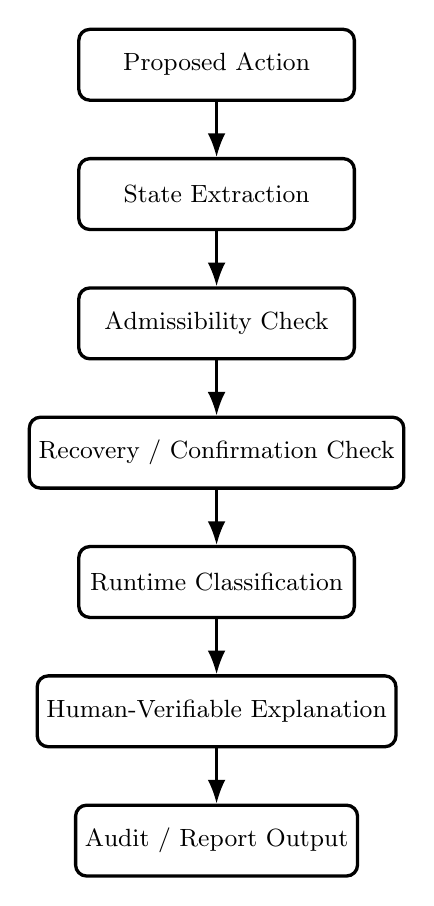
\begin{tikzpicture}[node distance=7mm]
\node[block] (a) {Proposed Action};
\node[block, below=of a] (b) {State Extraction};
\node[block, below=of b] (c) {Admissibility Check};
\node[block, below=of c] (d) {Recovery / Confirmation Check};
\node[block, below=of d] (e) {Runtime Classification};
\node[block, below=of e] (f) {Human-Verifiable Explanation};
\node[block, below=of f] (g) {Audit / Report Output};

\draw[arrow] (a) -- (b);
\draw[arrow] (b) -- (c);
\draw[arrow] (c) -- (d);
\draw[arrow] (d) -- (e);
\draw[arrow] (e) -- (f);
\draw[arrow] (f) -- (g);
\end{tikzpicture}
\caption{v3.8 runtime governance refinement pipeline.}
\end{figure}

This can be modeled as function composition:

\[
G(T)
=
Classify
\circ
Confirm
\circ
Recover
\circ
Check
\circ
Extract
(S_t,T).
\]

Define:

\[
X_t = Extract(S_t,T),
\quad
A_t = Check_C(X_t),
\quad
R_t = Recover(A_t,T),
\]

\[
H_t = Confirm(R_t),
\quad
G_t = Classify(H_t),
\]

\[
Report_t = Explain(G_t,X_t,C,R_t,H_t).
\]

% ============================================================
\section{\texorpdfstring{\mbox{v4.0}: Bounded Permission}{v4.0: Bounded Permission}}

v4.0 introduces the principle:

\[
\GO \neq \text{Unlimited Permission}.
\]

Instead:

\[
\GO = \text{Bounded Permission}.
\]

Let \(K\) denote an execution contract.

\[
K =
\{
allowed\_action,
allowed\_target,
allowed\_scope,
prohibited\_actions,
preconditions,
audit\_required,
human\_confirmation
\}.
\]

\[
\GO(T)
\Rightarrow
\exists K : Bound(T,K)=1.
\]

Therefore:

\[
BoundedPermit(T,K)
=
\mathbf{1}
\left[
C(S_t,T,S_{t+1})=1
\land
Bound(T,K)=1
\right].
\]

\begin{figure}[H]
\centering
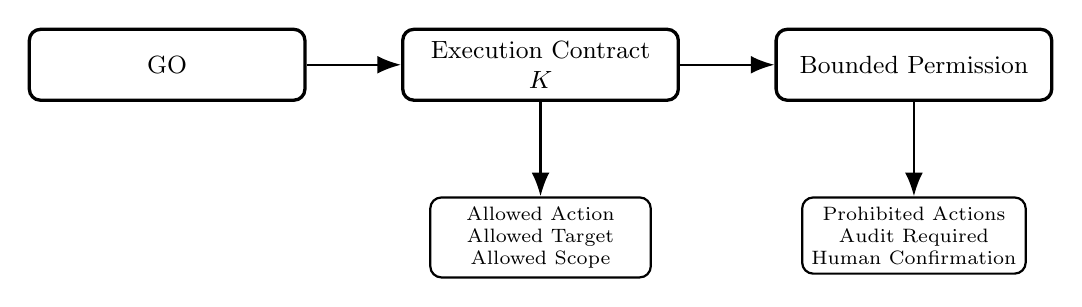
\begin{tikzpicture}[node distance=12mm]
\node[block] (go) {GO};
\node[block, right=of go] (contract) {Execution Contract\\\(K\)};
\node[block, right=of contract] (bounded) {Bounded Permission};

\node[smallblock, below=of contract] (allow) {Allowed Action\\Allowed Target\\Allowed Scope};
\node[smallblock, below=of bounded] (deny) {Prohibited Actions\\Audit Required\\Human Confirmation};

\draw[arrow] (go) -- (contract);
\draw[arrow] (contract) -- (bounded);
\draw[arrow] (contract) -- (allow);
\draw[arrow] (bounded) -- (deny);
\end{tikzpicture}
\caption{In v4.0, GO is converted into bounded permission through an execution contract.}
\end{figure}

% ============================================================
\section{Execution Contract Enforcement}

Let \(E\) denote the attempted execution.
Let \(K\) denote the issued execution contract.

\[
Enforce(E,K)
\in
\{\PASS,\VIOLATION\}.
\]

\[
Enforce(E,K)=\PASS
\iff
E\subseteq K.
\]

\[
Enforce(E,K)=\VIOLATION
\iff
E\nsubseteq K.
\]

\begin{table}[H]
\centering
\caption{Contract enforcement examples.}
\begin{tabular}{p{0.28\linewidth} p{0.34\linewidth} p{0.22\linewidth}}
\toprule
\textbf{Contract \(K\)} & \textbf{Attempt \(E\)} & \textbf{Result} \\
\midrule
Read \(file_A\) & Read \(file_A\) & \(\PASS\) \\
Read \(file_A\) & Read \(file_A\) + Upload \(file_A\) & \(\VIOLATION\) \\
Write \(summary.md\) & Overwrite \(README.md\) & \(\VIOLATION\) \\
Delete confirmed temp files & Delete project directory & \(\VIOLATION\) \\
\bottomrule
\end{tabular}
\end{table}

% ============================================================
\section{\texorpdfstring{\mbox{v4.0} Closed-Loop Governance}{v4.0 Closed-Loop Governance}}

The v4.0 closed-loop governance flow is:

\begin{figure}[H]
\centering
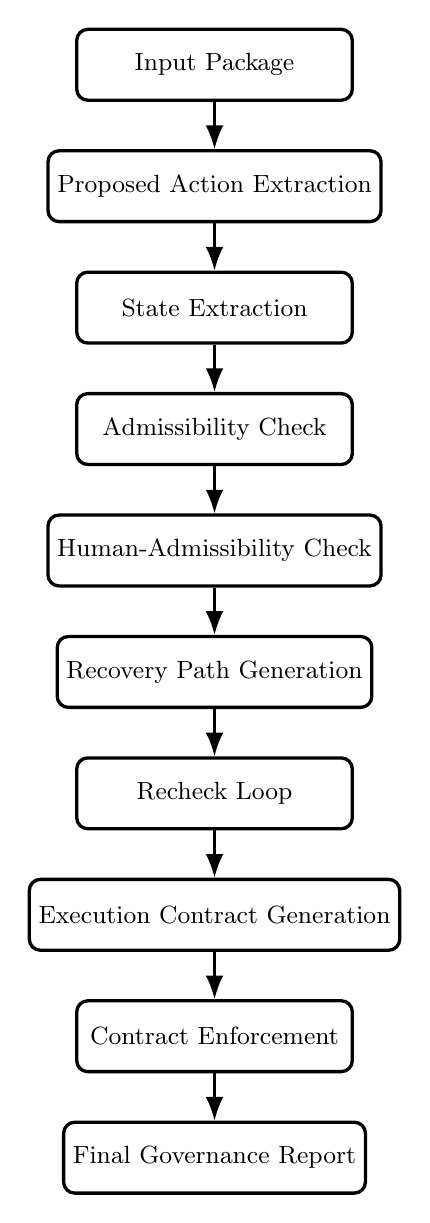
\begin{tikzpicture}[node distance=6mm]
\node[block] (input) {Input Package};
\node[block, below=of input] (extract) {Proposed Action Extraction};
\node[block, below=of extract] (state) {State Extraction};
\node[block, below=of state] (check) {Admissibility Check};
\node[block, below=of check] (human) {Human-Admissibility Check};
\node[block, below=of human] (recovery) {Recovery Path Generation};
\node[block, below=of recovery] (recheck) {Recheck Loop};
\node[block, below=of recheck] (contract) {Execution Contract Generation};
\node[block, below=of contract] (enforce) {Contract Enforcement};
\node[block, below=of enforce] (report) {Final Governance Report};

\draw[arrow] (input) -- (extract);
\draw[arrow] (extract) -- (state);
\draw[arrow] (state) -- (check);
\draw[arrow] (check) -- (human);
\draw[arrow] (human) -- (recovery);
\draw[arrow] (recovery) -- (recheck);
\draw[arrow] (recheck) -- (contract);
\draw[arrow] (contract) -- (enforce);
\draw[arrow] (enforce) -- (report);
\end{tikzpicture}
\caption{v4.0 stable closed-loop runtime governance pipeline.}
\end{figure}

Define:

\[
X = Extract(S_t,T),
\quad
a = C(X),
\quad
r = Recovery(T),
\]

\[
T' = Recheck(r(T)),
\quad
K = Contract(T'),
\quad
e = Enforce(E,K),
\]

\[
\FGR = FinalGovernanceReport(X,a,r,T',K,e).
\]

% ============================================================
\section{\texorpdfstring{\mbox{v4.1} Contract Violation Response}{v4.1 Contract Violation Response}}

v4.1 defines how the system responds when execution violates the issued contract.

Let:

\[
V=Violation(E,K).
\]

Let severity be:

\[
\sigma(V)
\in
\{\mathrm{LOW},\mathrm{MEDIUM},\mathrm{HIGH},\mathrm{CRITICAL}\}.
\]

Let response selection be:

\[
\lambda(V)
\in
\{\OBSERVE,\PAUSE,\REPAIR,\ROLLBACK,\ESCALATE,\BLOCK\}.
\]

If:

\[
Enforce(E,K)=\VIOLATION,
\]

then:

\[
\lambda(V)
=
SelectResponse(\sigma(V),Context,Policy).
\]

\begin{figure}[H]
\centering
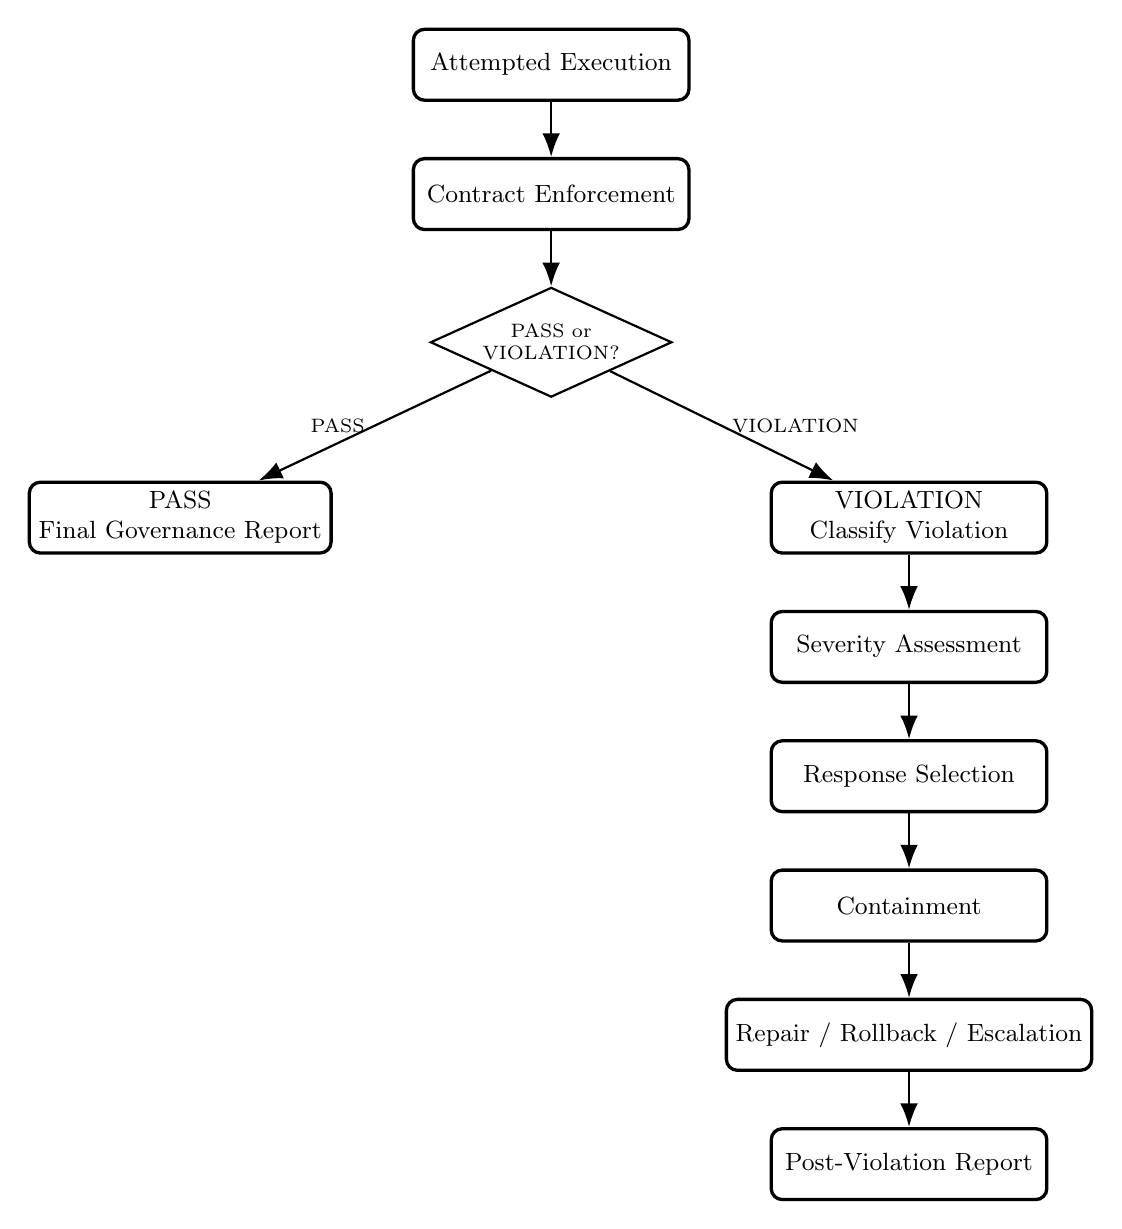
\begin{tikzpicture}[node distance=7mm]
\node[block] (attempt) {Attempted Execution};
\node[block, below=of attempt] (enforce) {Contract Enforcement};
\node[decision, below=of enforce] (passvio) {PASS or\\VIOLATION?};

\node[block, below left=14mm and 20mm of passvio] (pass) {PASS\\Final Governance Report};
\node[block, below right=14mm and 20mm of passvio] (vio) {VIOLATION\\Classify Violation};

\node[block, below=of vio] (severity) {Severity Assessment};
\node[block, below=of severity] (response) {Response Selection};
\node[block, below=of response] (contain) {Containment};
\node[block, below=of contain] (repair) {Repair / Rollback / Escalation};
\node[block, below=of repair] (pvr) {Post-Violation Report};

\draw[arrow] (attempt) -- (enforce);
\draw[arrow] (enforce) -- (passvio);
\draw[arrow] (passvio) -- node[left, font=\scriptsize] {PASS} (pass);
\draw[arrow] (passvio) -- node[right, font=\scriptsize] {VIOLATION} (vio);
\draw[arrow] (vio) -- (severity);
\draw[arrow] (severity) -- (response);
\draw[arrow] (response) -- (contain);
\draw[arrow] (contain) -- (repair);
\draw[arrow] (repair) -- (pvr);
\end{tikzpicture}
\caption{v4.1 contract violation response flow.}
\end{figure}

% ------------------------------------------------------------
\subsection{Violation Severity}

Violation risk can be modeled as:

\[
Risk(V)
=
w_dD
+
w_eE_{\mathrm{ext}}
+
w_cCred
+
w_gGov
+
w_iIrrev
+
w_sScope
+
w_hHuman.
\]

Severity is thresholded as:

\[
\sigma(V)=
\begin{cases}
\mathrm{LOW}, & Risk(V)<\theta_1,\\
\mathrm{MEDIUM}, & \theta_1\leq Risk(V)<\theta_2,\\
\mathrm{HIGH}, & \theta_2\leq Risk(V)<\theta_3,\\
\mathrm{CRITICAL}, & Risk(V)\geq \theta_3.
\end{cases}
\]

% ------------------------------------------------------------
\subsection{Response Selection}

\[
\lambda(V)
=
SelectResponse
\left(
\sigma(V),
Recoverable(V),
ExternalEffect(V),
CredentialRisk(V),
GovernanceBypass(V)
\right).
\]

\begin{table}[H]
\centering
\caption{Severity-to-response matrix.}
\begin{tabular}{p{0.18\linewidth} p{0.40\linewidth} p{0.28\linewidth}}
\toprule
\textbf{Severity} & \textbf{Typical Condition} & \textbf{Default Response} \\
\midrule
LOW & Minor boundary deviation without state change & \(\OBSERVE / \PAUSE\) \\
MEDIUM & Scope expansion or unsafe modification attempt & \(\PAUSE / \REPAIR\) \\
HIGH & External effect, destructive attempt, sensitive action & \(\ESCALATE / \BLOCK\) \\
CRITICAL & Credential exposure, destructive deletion, governance bypass & \(\BLOCK\) \\
\bottomrule
\end{tabular}
\end{table}

% ============================================================
\section{Post-Violation Report}

A post-violation report is generated when contract enforcement fails.

\[
\PVR
=
ReportViolation
(K,E,V,\sigma(V),\lambda(V),Containment,Rollback,Repair,Audit).
\]

Its content is represented as:

\[
\PVR
=
\{
contract\_id,
attempted\_action,
allowed\_action,
violated\_rule,
severity,
response\_level,
containment\_status,
rollback\_status,
repair\_option,
human\_review\_required,
final\_recommendation,
audit\_trace
\}.
\]

\begin{table}[H]
\centering
\caption{Post-violation report fields.}
\begin{tabular}{p{0.30\linewidth} p{0.58\linewidth}}
\toprule
\textbf{Field} & \textbf{Meaning} \\
\midrule
contract\_id & Identifier of the issued execution contract. \\
attempted\_action & Action attempted during execution. \\
allowed\_action & Action originally allowed by the contract. \\
violated\_rule & Contract rule that was violated. \\
severity & LOW / MEDIUM / HIGH / CRITICAL. \\
response\_level & OBSERVE / PAUSE / REPAIR / ROLLBACK / ESCALATE / BLOCK. \\
containment\_status & How execution was contained. \\
rollback\_status & Whether rollback was possible or required. \\
repair\_option & Possible safer path, if available. \\
audit\_trace & Human-verifiable record of governance events. \\
\bottomrule
\end{tabular}
\end{table}

% ============================================================
\section{Integrated Output Function}

Let \(\FGR\) denote the Final Governance Report.
Let \(\PVR\) denote the Post-Violation Report.

\[
Output(T)
=
\begin{cases}
\FGR(T,K,E), & Enforce(E,K)=\PASS,\\
\PVR(T,K,E,V), & Enforce(E,K)=\VIOLATION.
\end{cases}
\]

% ============================================================
\section{General Abstract Model}

I2OS Mini Gate can be abstractly defined as:

\[
\MG
=
\langle
S,T,C,G,\rho,K,E,V,\sigma,\lambda,R
\rangle.
\]

\begin{longtable}{p{0.20\linewidth} p{0.70\linewidth}}
\toprule
\textbf{Symbol} & \textbf{Meaning} \\
\midrule
\(S\) & State space. \\
\(T\) & Set of possible transitions. \\
\(C\) & Admissibility constraint. \\
\(G\) & Classification function: \(\GO/\HOLD/\REPAIR/\BLOCK\). \\
\(\rho\) & Repair mapping. \\
\(K\) & Execution contract. \\
\(E\) & Attempted execution. \\
\(V\) & Contract violation. \\
\(\sigma\) & Violation severity function. \\
\(\lambda\) & Violation response function. \\
\(R\) & Report generation function. \\
\bottomrule
\end{longtable}

The full operation can be expressed as:

\[
I2OS\_MG(T)
=
R
\left(
\lambda
\left(
\sigma
\left(
V
\left(
E,
K
\left(
\rho
\left(
C
\left(
Extract(S_t,T)
\right)
\right)
\right)
\right)
\right)
\right)
\right).
\]

\[
Extract
\rightarrow
Check
\rightarrow
Classify
\rightarrow
Repair
\rightarrow
Contract
\rightarrow
Enforce
\rightarrow
Respond
\rightarrow
Report.
\]

% ============================================================
\section{Admissible Action Space}

Let \(\mathcal{T}\) be the set of possible transitions.

The admissible transition set is:

\[
\mathcal{T}_{allow}
=
\{
T\in\mathcal{T}
\mid
C(S_t,T,S_{t+1})=1
\}.
\]

The executable transition set under v4.0 and v4.1 is:

\[
\mathcal{T}_{execute}
=
\{
T\in\mathcal{T}
\mid
C(T)=1
\land
Bound(T,K)=1
\land
Enforce(E,K)=\PASS
\}.
\]

If:

\[
E\nsubseteq K,
\]

then:

\[
E\nsubseteq K
\Rightarrow
V
\Rightarrow
\sigma(V)
\Rightarrow
\lambda(V)
\Rightarrow
\PVR.
\]

% ============================================================
\section{Final Formal Definition}

\begin{definition}[I2OS Mini Gate]
I2OS Mini Gate is a closed-loop runtime governance system that extracts proposed AI/software actions as state transitions before execution, classifies them according to admissibility constraints, converts permitted transitions into bounded execution contracts, enforces those contracts during attempted execution, and responds to contract violations through severity classification, containment, repair, rollback, escalation, blocking, and human-verifiable reporting.
\end{definition}

Formally:

\[
I2OS\_MG
:
(S_t,T)
\mapsto
\begin{cases}
\FGR, & C(T)=1 \land Bound(T,K)=1 \land E\subseteq K,\\
\PVR, & E\nsubseteq K,\\
\HOLD, & C_{\mathrm{core}}(T)=1 \land C_{\mathrm{human}}(T)=0,\\
\REPAIR, & C(T)=0 \land \exists \rho : C(\rho(T))=1,\\
\BLOCK, & C(T)=0 \land \neg\exists \rho : C(\rho(T))=1.
\end{cases}
\]

% ============================================================
\section{Ultra-Compact Form}

The shortest expression of I2OS Mini Gate is:

\[
\mathrm{Capability} \neq \mathrm{Permission}.
\]

Permission is defined as:

\[
\text{Permission}
=
\text{Admissibility}
\land
\text{Boundedness}
\land
\text{Recoverability}
\land
\text{Human Verifiability}.
\]

A safe AI action is:

\[
\text{Safe AI Action}
=
\text{Permitted Transition}
+
\text{Bounded Contract}
+
\text{Violation Response}.
\]

Equivalently:

\[
\text{Safe AI Action}(T)
=
C(T)
\land
Bound(T,K)
\land
Response(V).
\]

% ============================================================
\section{Conclusion}

I2OS Mini Gate formalizes a shift from output filtering to runtime transition governance.

The system does not merely ask whether an AI can act.
It asks whether a proposed transition is admissible before execution, whether permission is bounded during execution, and how governance should respond after violation.

Thus:

\[
\text{AI Safety}
=
\text{Pre-Execution Governance}
+
\text{Bounded Execution}
+
\text{Post-Violation Response}.
\]

In natural language:

\begin{quote}
AI safety is not only output filtering.

It is admissible transition governance before action,
bounded permission during execution,
and structured response after violation.
\end{quote}

\begin{quote}
Safe intelligence is not intelligence that never collapses.

Safe intelligence is intelligence that can recursively re-synchronize.
\end{quote}

\end{document}
